%%%  P9_latex09_LaTeX中的浮动体
% 导言区
\documentclass{ctexart}%ctexbook, ctexrep

%\usepackage{ctex}
%\usepackage{graphics}
\usepackage{graphicx}
\graphicspath{{pictures/}} % 图片在当前目录下的figures 目录

% 正文区(文稿区)
\begin{document}
	\LaTeX{}中\TeX 系统的吉祥物---小狮子见图\ref{fig-lion}:
	\begin{figure}[htbp]
		\centering
		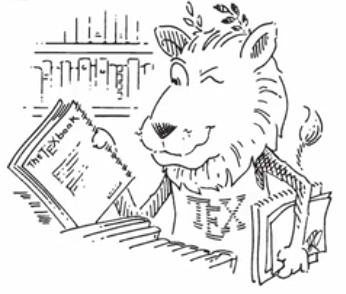
\includegraphics[scale=0.3]{lion.png}
		\caption{\TeX 系统的吉祥物---小狮子}\label{fig-lion}
	\end{figure}
	
%	遥望太白,看积雪皑皑,别有一番风景(图\ref{fig-mountain})。
%	\begin{figure}[htbp]
%		\centering
%		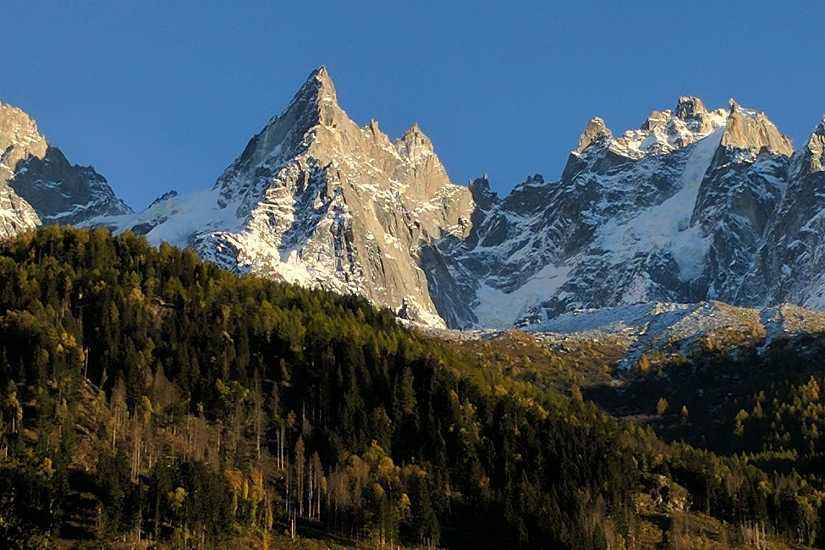
\includegraphics[scale=0.3]{mountain.jpg}
%		\caption{太白山}\label{fig-mountain}
%	\end{figure}

	熟练使用\LaTeX 中的TiKz,可以绘制如图\ref{fig-tikz}所示的精美矢量图。
	\begin{figure}[htbp]
		\centering
		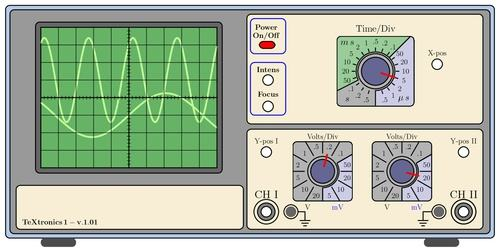
\includegraphics[scale=0.3]{oscilloscope}
		\caption{\LaTeX 中的矢量图}\label{fig-tikz}
	\end{figure}
	
	当然,在\LaTeX{}中也可以使用表\ref{tab-score}所示的表格。
	\begin{table}[h]
		\centering
		\caption{考试成绩单}\label{tab-score}
		\begin{tabular}{l|c|c|c|r}
			\hline
			姓名 & 语文 & 数学 & 外语 & 备注 \\
			\hline \hline
			张三 & 87 & 100 & 93 & 优秀 \\
			\hline
			李四 & 75 & 64 & 52 & 补考另行通知 \\
			\hline
			王二 & 80 & 82 & 78 & \\
			\hline
		\end{tabular}
	\end{table}
	
\end{document}

